\documentclass[a4paper,12pt]{article}
\usepackage{mathptmx}
\usepackage{enumitem} 
\usepackage{geometry}
\usepackage{amsmath}
\usepackage{setspace}
\usepackage{graphicx}
\usepackage{caption}
\usepackage{float}
\usepackage{amsfonts}
\usepackage{amssymb}
\usepackage{hyperref}
\usepackage{listings}
\usepackage{color}
\usepackage[utf8]{inputenc}  
\usepackage{cite}  
\usepackage{indentfirst}

\geometry{margin=1in}

\begin{document}

\begin{titlepage}
    \centering
    
\includegraphics[width=8cm]{Images/Nanyang_Technological_University-Logo.wine.png}\par\vspace{1cm}
    {\scshape\LARGE Nanyang Technological University \par}
    \vspace{1.5cm}
    {\huge\bfseries EE6222 Machine Vision\par}
    \vspace{0.5cm}
    {\Large Assignment 1: Dimensionality Reduction for Classification\par}
    \vspace{2cm}
    {\large MSc in Electrical and Electronic Engineering\par}
    {\large Yan Ziming\par}
    {\large G2507084J\par}
    \vfill
    {\large \today \par}
\end{titlepage}

\newpage
\tableofcontents
\newpage

\section{Introduction}
In this Assignment, I selected the MINIST dataset for training and testing the performance of classifiers. As for the dimension of images are largee,
I explored several dimensionality reduction methods to reduce the dimension of data while trying to retain the most important features, including \textbf{PCA}, \textbf{LDA}, 
combined method (Fisherfaces), \textbf{LLE}, \textbf{Isomap}, and \textbf{PaCMAP}. I compared the effectiveness of these methods by plotting their performance with varying number of
dimensions. 

In addition, I establish several basic classifiers, like \textbf{MMD}, \textbf{KNN}, and include Logistic Regression Classifier with sklearn package. Therefore, I not only 
compare the effectiveness of different dimensionality reduction methods, but also access the accuracy of classifiy images for these classifer methods. I would 
describe the details of my experiment in the fllowing sections.  

\section{Dataset and Preprocessing}
\subsection{Dtaset Descrption}
The MINIST dataset contains \textbf{70,000} images of handwritten digits (0-9) with a resolution of 28x28 pixels, which means there are \textbf{10} classes intotal. Each image had been saved with the 
format of vector with \textbf{784 in length}. In addition, the images are only have one channel, which means they are grayscale pixels. Because of the pre-shaped vectors, single channel, and 
easy to get features, I think MINIST dataset is suitable for this assignment.
Therefore, I fetch the dataset from sklearn package directly \ref{fig:fetch}.
\begin{figure}[H]
    \centering
    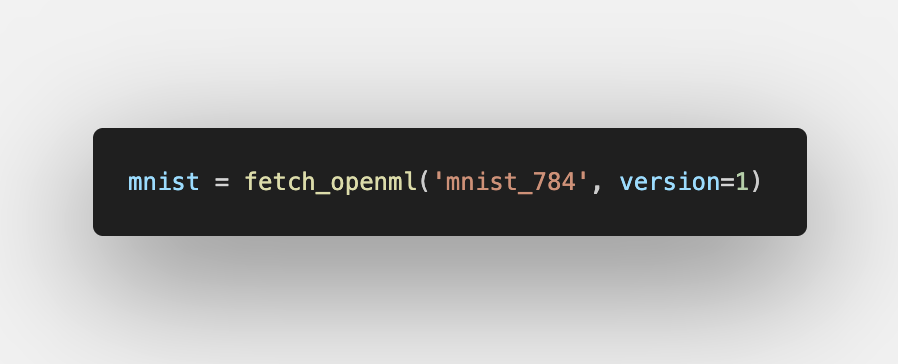
\includegraphics[width=0.8\textwidth]{Images/MINIST_fetch.png}
    \caption{Fetch Code}
    \label{fig:fetch}
\end{figure}
\subsection{Normalization and Standarlization}
Since the MINIST dataset had been well preprocessed and tested by plenty of researchers, I didn't do too much basic preprocessing, like outlier and missing value detection. However, I though normalization and 
standarlization arer still neccessary for the following basic classifiers, which may be affected intensely by the scle of features. So I rearrange the vectors to 0 mean and unit variance.
\[
    \bar X=\frac{X}{L-1}
\]
\[
    X_{std}=\frac{X-\mu}{\sigma}
\]
\subsection{Dataset Partition}
I found the number of samples (70,000) is too large, which may lead to many difficulties in my following experiment. Firstly, I will traing several classifiers with many dimension reduction methods, 
meaning the number of training process will be big. If I train 50,000-70,000 for each training, the consummed time will be very long. Secondly, my classifers which will be used are simple and bisic, therefore, they are 
easy to converge with small scale of data. With these two reason, I deciode to extract 7,000 samples from the origin dataset formly to reduce the expence of time.

After that, I split the dataset into training set and testing set through \textit{\textbf{train\_test\_split}} function with ratio of 6:1 and finished the process of preparation of dataset \ref{fig:datapartition}.
\begin{figure}[H]
    \centering
    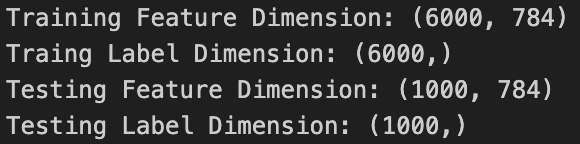
\includegraphics[width=0.6\textwidth]{Images/Datapartition.png}
    \caption{Dimension of practical dataset}
    \label{fig:datapartition}
\end{figure}
\section{Methodology}

\subsection{Linear Dimensionality Reduction}
\subsubsection{Linear Discriminant Analysis}
Linear Discriminant Analysis (LDA) aims to find a linear combination of features with weight matrix $\mathbf{w}$ to transform the data into linear space, ensuring that the seperation between different 
classes is maximized while the variance with each class is minimized.
\vspace{0.5cm}

\noindent \textit{\textbf{Step 1: Mean Value Computation}}

With given m classes \{$w_1$, $w_2$, ... $w_m$\}, there are c samples in each class w: \{$X_1$, $X_2$, ... $X_c$\}. For each sample vector, it has n features, \{$x_1$, $x_2$, ... , $x_n$\}. In this experiment, \textbf{n=784}.

Overall Mean:
\[
    \mu_t = \frac{1}{N}\sum_{i=1}^{N} x_i
\]

Class Mean:
\[
    \mu_i = \frac{1}{n_i}\sum_{j=1}^{n_i} x_j
\]

Where $N$ is the total number of samples, and $n_i$ is the number of samples in class $w_i$.

\vspace{0.5cm}
\noindent \textit{\textbf{Step 2: Scatter Matrix Computation}}

Between-Class Scatter Matrix:
\[
    S_B=n_i*\sum_{j=1}^{m}(\mu_j-\mu_t)(\mu_j-\mu_t)^T
\]

Within-Class Scatter Matrix:
\[
    S_W=\sum_{j=1}^{m}\sum_{x_i \in w_j}(x_i-\mu_j)(x_i-\mu_j)^T
\]
\begin{figure}[H]
    \centering
    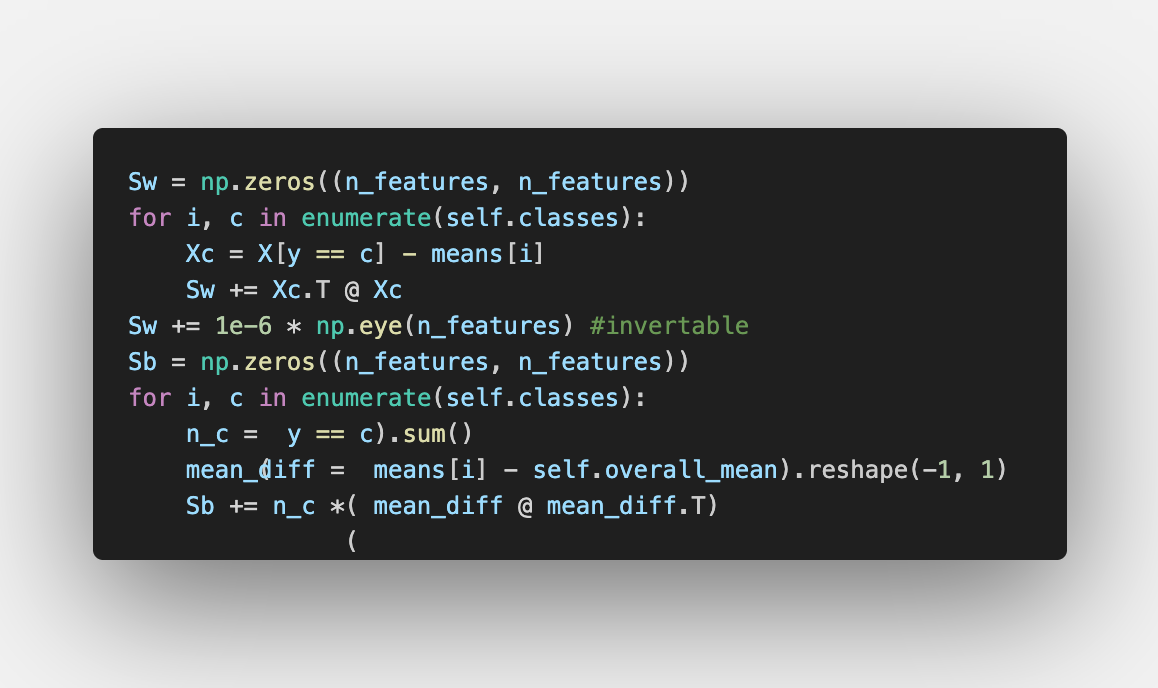
\includegraphics[width=0.8\textwidth]{Images/LDA_scatter_compute.png}
    \caption{Scatter Computation Code}
    \label{fig:S_C}
\end{figure}
\noindent \textit{\textbf{Step 3: Weight Matrix Computation}}

As I mentioned before, the LDA aims to find the optimal weight matrix to seperate classes on two dimension, equaling to the problem: maximize the ratio of between-class scatter to within-class scatter.
\begin{equation}
    \mathbf{w}^*=\mathop{\arg\max}\limits_{w}\frac{|w^TS_Bw|}{|w^TS_Ww|}
\end{equation} 

Since the $S_Bw_i=\lambda_iS_Ww_i$,
\begin{equation}
    \lambda\mathbf{w}=S_W^{-1}S_B\mathbf{w}
\end{equation}

Therefore, the $\mathbf{w}$ is the eigenvectors matrix according to eigenvalue $\lambda$, the largest $\lambda$ refers to best matrix $\mathbf{w}^*$.

\begin{figure}[H]
    \centering
    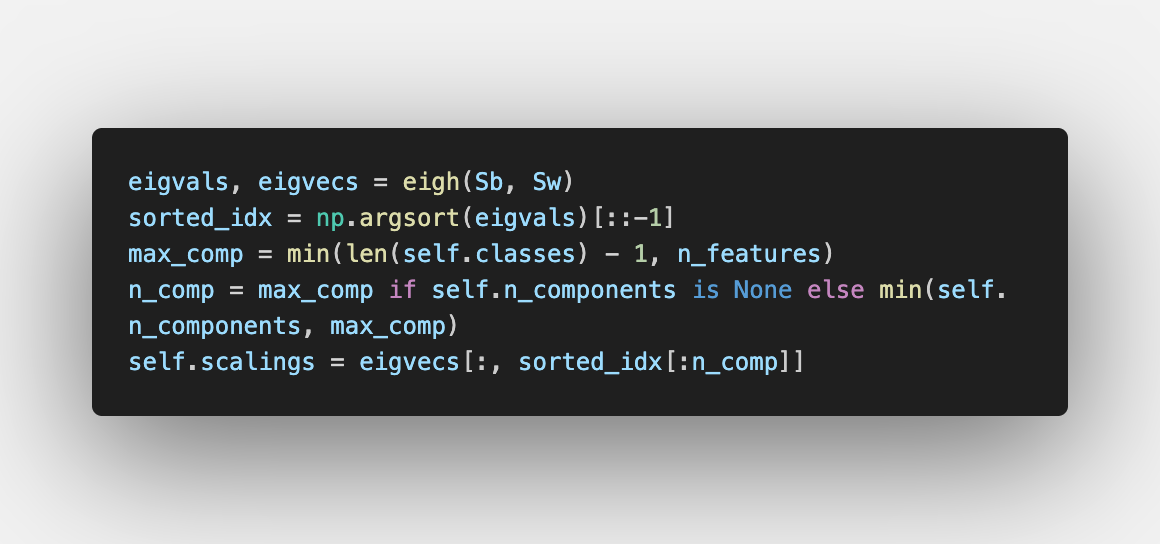
\includegraphics[width=0.8\textwidth]{Images/LDA_weight_compute.png}
    \caption{Eigenvector Matrix Computation}
    \label{fig:E_M_C}
\end{figure}
\noindent \textit{\textbf{Step 4: Transform Dataset}}

After getting the weight matrix, the transformation of input data $\mathbf{X}$ is:
\[
    \mathbf{Y} = \mathbf{X}\mathbf{w}^*
\]

In practice, we will choose the $k^{th}$ value of sorted eigenvalues to form $\mathbf{w}^*$. Theoritically, LDA is designed to project samples onto 
a lower-dimensional subspace, with the dimensionality being at most C - 1, because the rank of $S_B$ is at most C-1, C is the number of classes.

\subsubsection{Principal Component Analysis}
Similar to LDA, Principal Component Analysis (PCA) is another effective method to dimensionality reduction. The difference is PCA can project the input data to 
different dimensions without limitaion like LDA. The projected data after PCA will also seperate largly, which means the redundency elements are eliminated.

\vspace{0.5cm}
\noindent \textit{\textbf{Step 1: Data Processing}}

Before the projection, the data should be scaled and normalized, eliminating bias. Specifically, compute mean value to shift to 0 mean and covariance to 
investigate the distribution situation of data.

Covariance Matrix Computation:
\[
    \Sigma_i=\sum_{x_j \in w_i}^{n_i}(x_j-\mu_i)(x_j-\mu_i)^T
\]

Where $\mu_i$ is the mean value of class $w_i$

\vspace{0.5cm}
\noindent \textit{\textbf{Step 2: Eigenvectors Computation}}

The PCA aims to find the direction $\mathbf{w}$, the variance of data projected to that direction is largest. For the transformed data $Y=\mathbf{w}X$, variance computed:
\[
    Var(Y)=\frac{1}{N}\sum_{i=1}^N(w^Tx_i)^2=w^T\Sigma w
\]

Solving the $\mathop{\arg\max}\limits_{w}(w^T\Sigma w)$,
\begin{equation}
    \Sigma \mathbf{w}=\lambda \mathbf{w}
\end{equation}

Larger eigenvalue refers to better eigenvector, by sort the eigenvalues in descending sequence, we can fetch $k^{th}$ large vlues and their correspondingly eigenvectors to form best
matrix $\mathbf{w}^*$.
\begin{figure}[H]
    \centering
    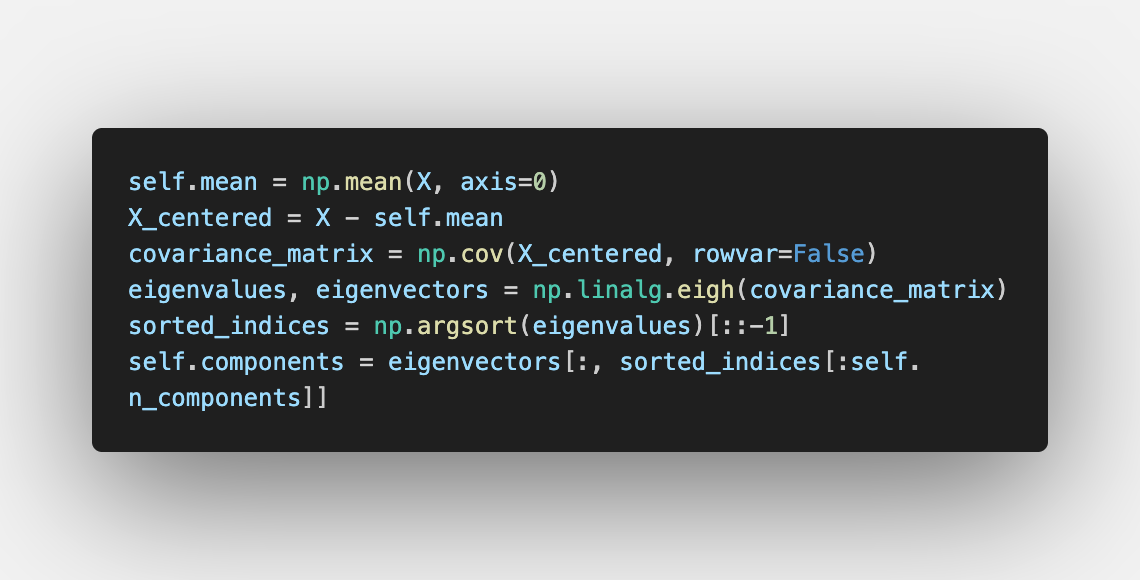
\includegraphics[width=0.8\textwidth]{Images/PCA.png}
    \caption{PCA Realization Code}
    \label{fig:PCA}
\end{figure}

\noindent \textit{\textbf{Step 3: Transform Dataset}}

With above process, we can get the corresponding optimal weight matrix, according to the input data and componenet coefficient k. Applying the matrix to input data, transformation finished.

\subsubsection{Fisherfaces}

Based on learning in course, I acknowledge that the reduction of feature equals to deleting redundant features, which can increase the accuray of models. However, when too much features deleted, the remaining features 
may not includes all the information we need, which causes the decrease of accuray backward. Therefore, the best accuarcy of LDA towards high dimension data is much lower than PCA normally. To overcome this situation, 
the Fisherfaces, which combines the LDA and PCA method is developed.

For realization, I just handle the data with PCA to roughly decrease the dimension firstly. Then, I applied LDA based on the corresponding PCA space to finish the whole reduction.
\subsection{Nonlinear Dimensionality Reduction}
% \noindent \textit{\textbf{Manifold Definition:}} 
 
A \textbf{manifold} is a topological space that locally resembles Euclidean space. 
Intuitively, even if data lie in a high-dimensional ambient space $\mathbb{R}^D$, 
their intrinsic degrees of freedom may be much smaller, forming a $d$-dimensional manifold $(d \ll D)$. 
For example, images of a rotating object under fixed lighting conditions can be considered points on a 2D manifold embedded in a high-dimensional pixel space.

Formally, a dataset $X = \{x_1, x_2, \ldots, x_N\}$ is assumed to lie on or near a smooth manifold $\mathcal{M}$ of dimension $d$. 
The goal of \textbf{manifold learning} is to find a mapping $f: \mathbb{R}^D \to \mathbb{R}^d$ that preserves intrinsic geometric relationships among points.

Unlike linear methods such as PCA, which only capture global linear structures, manifold learning methods exploit the underlying nonlinear geometry. I include manifold learning methods for 
dimension reduction in this experiment.
\subsubsection{Locally Linear Embedding}
\noindent \textit{\textbf{Brief Introduction:}}

Locally Linear Embedding (LLE) is a nonlinear dimensionality reduction algorithm that preserves local geometric relationships between neighboring data points. 
It assumes that each data point and its neighbors lie on or close to a locally linear manifold. 
LLE first reconstructs each data point as a linear combination of its nearest neighbors in the original high-dimensional space, then seeks a low-dimensional embedding that maintains these same reconstruction weights \cite{lle}.

Let the dataset be $\{x_1, x_2, \ldots, x_N\}$, where each $x_i \in \mathbb{R}^D$. 
For each data point $x_i$, find its $K$ nearest neighbors $\mathcal{N}(i)$ using Euclidean distance. 
Each point is reconstructed from its neighbors:
\[
x_i \approx \sum_{j \in \mathcal{N}(i)} w_{ij} x_j
\]

The reconstruction weights $w_{ij}$ are obtained by minimizing the local reconstruction error:
\begin{equation}
\min_{W} \sum_{i=1}^{N} \left\| x_i - \sum_{j \in \mathcal{N}(i)} w_{ij} x_j \right\|^2
\end{equation}

subject to the constraint:
\[
\sum_{j \in \mathcal{N}(i)} w_{ij} = 1
\]

These weights capture the intrinsic geometry of the data.

In the embedding step, we find low-dimensional representations $y_i \in \mathbb{R}^d$ $(d \ll D)$ that preserve the same reconstruction weights:
\begin{equation}
\min_{Y} \sum_{i=1}^{N} \left\| y_i - \sum_{j \in \mathcal{N}(i)} w_{ij} y_j \right\|^2
\end{equation}

subject to:
\[
\sum_i y_i = 0, \quad \frac{1}{N}\sum_i y_i y_i^T = I
\]

The optimal embedding $Y = [y_1, \ldots, y_N]^T$ is obtained by computing the bottom $(d+1)$ eigenvectors of the matrix:
\begin{equation}
M = (I - W)^T (I - W)
\end{equation}

and discarding the smallest eigenvector corresponding to the zero eigenvalue.

\vspace{0.5cm}
\noindent \textit{\textbf{Implementation:}}

In this experiment, I implemted the LLE by using the \texttt{LocallyLinearEmbedding} class from \texttt{scikit-learn}. 
The key parameters are the number of neighbors (\texttt{n\_neighbors}) and the target embedding dimension (\texttt{n\_components}).  
Below shows an example code used in this experiment:
\begin{figure}[H]
    \centering
    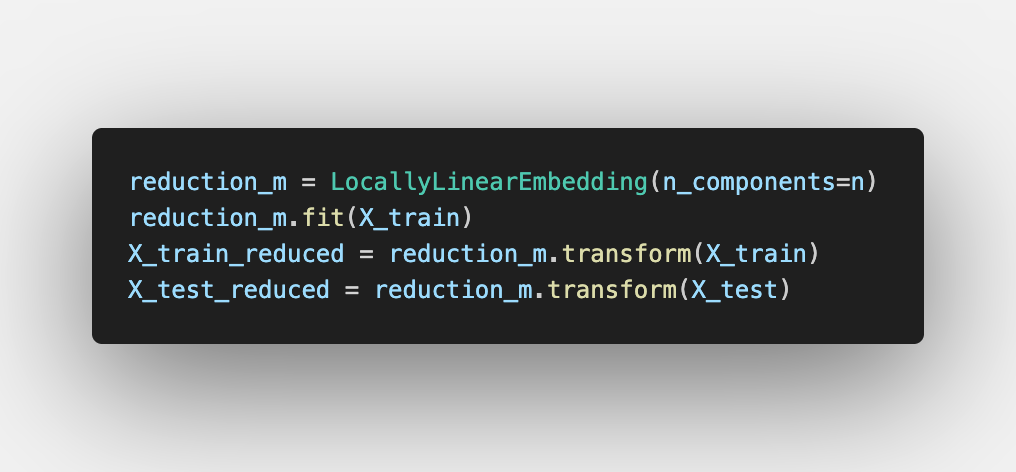
\includegraphics[width=0.8\textwidth]{Images/lle.png}
    \caption{LLE Realization Code}
    \label{fig:lle}
\end{figure}
\subsubsection{Isometric Mapping}
\noindent \textit{\textbf{Brief Introduction:}}
\cite{isomap}
\subsubsection{Pairwise Controlled Manifold Approximation}

\subsection{Classifiers Establishment}
\subsubsection{Minimun Mahalanobis Distance Classifier}
\subsubsection{K-Nearest Neighbors Classifier}
\subsubsection{Logistic Regression Classifier}

\subsection{Evaluation Methods}


\section{Results and Discussion}

\section{Conclusion}


\newpage
\bibliographystyle{ieeetr}
\bibliography{references}
\newpage
\section*{Appendix}
\end{document}